\section{\textsc{Whipped omelette}}

\subsection*{Ingredients for 2 omelettes:}

\begin{tabular}{p{7.5cm} p{7.5cm}}
	& \\
	8 eggs & 4 vienna sausages \\
	1 onion & 400g mozzarella \\
	salt und pepper &
\end{tabular}

\subsection*{Serving suggestion:}

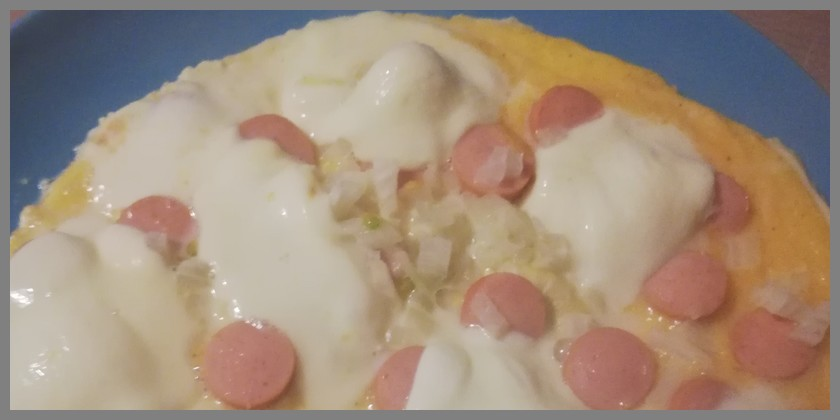
\includegraphics[width=\textwidth]{img/omlett_gewienert.jpg} \cite{omlettwiener}

\subsection*{How it's done:}

\begin{tabular}{p{15cm}}
  \\
  Beat the eggs in a bowl until foamy.\\
  Melt the butter in a large pan.\\
  In the meantime, cut the sausages into thin slices.\\
  Finely dice the onions.\\
  Pour the egg mixture into the pan and let it set over a high heat.\\
  Spread the sausages and the onions over the omelette.\\
  Fry with a lid on the pan for 5 minutes.\\
  Serve on a large plate.
\end{tabular}
